\section{Diagnosis}
\label{sec:diagnosis}

Table~\ref{tab:main_results} reports SICA vs.\ SC accuracy across all conditions. None of sixteen non-degenerate conditions shows a significant positive effect ($p < 0.05$); two show significant degradation. We trace this failure to three interconnected mechanisms.

\begin{table*}[t]
\centering
\small
\caption{SICA vs.\ SC across all conditions sorted by SC accuracy. $\Delta$ = SICA $-$ SC (pp). $^b$In-context learning with gold logical examples. $\dagger$\,$n < 100$ (suggestive only). \textbf{Bold $\Delta$}: $p < 0.05$ (McNemar). {*}\,$p < 0.05$;\enspace{**}\,$p < 0.01$;\enspace{***}\,$p < 0.001$. Failure modes detailed in Appendix~\ref{app:failure-modes}.}
\label{tab:main_results}
\begin{tabular}{@{}llrrrrl@{}}
\toprule
Model & Domain & $n$ & SC (\%) & SICA (\%) & $\Delta$ (pp) & $p$ \\
\midrule
\multicolumn{7}{l}{\textit{Type C: error amplification (SC $\leq$ 40\%)}} \\
Mistral-7B & PW-D5 & 600 & 39.33 & 36.50 & $\mathbf{-2.83}$ & 0.014{*} \\
\midrule
\multicolumn{7}{l}{\textit{Intermediate SC (SC $\sim$50--60\%, Mistral-7B only)}} \\
Mistral-7B & LogiQA & 200 & 50.00 & 51.50 & $+$1.50 & 0.581 \\
Mistral-7B & FOLIO (s123) & 204 & 54.41 & 57.35 & $+$2.94 & 0.070 \\
Mistral-7B & FOLIO & 204 & 55.88 & 59.31 & $+$3.43 & 0.092 \\
Mistral-7B & FOLIO (s456) & 204 & 55.88 & 55.88 & 0.00 & 1.000 \\
Mistral-7B & FOLIO (s789) & 204 & 59.31 & 56.86 & $-$2.45 & 0.267 \\
\midrule
\multicolumn{7}{l}{\textit{Type A: confirmation bias (SC $\geq$ 60\%)}} \\
LLaMA-3.1-8B & FOLIO & 204 & 66.18 & 61.76 & $-$4.41 & 0.093 \\
LLaMA-3.1-8B & StrategyQA & 200 & 72.00 & 74.00 & $+$2.00 & 0.424 \\
Qwen2.5-14B & FOLIO (ICL)$^b$ & 199 & 74.37 & 74.87 & $+$0.50 & 1.000 \\
Qwen2.5-14B & PW-D5 & 600 & 74.00 & 71.50 & $\mathbf{-2.50}$ & 0.011{*} \\
Qwen2.5-14B & FOLIO & 204 & 75.98 & 75.49 & $-$0.49 & 1.000 \\
Qwen2.5-7B & FOLIO & 204 & 75.98 & 76.47 & $+$0.49 & 1.000 \\
Qwen2.5-14B & LogiQA & 200 & 79.00 & 78.00 & $-$1.00 & 0.625 \\
Qwen3-14B & FOLIO & 204 & 83.33 & 84.80 & $+$1.47 & 1.000 \\
Qwen3-14B & PW-D5 & 600 & 85.83 & 85.67 & $-$0.17 & 1.000 \\
\midrule
\multicolumn{7}{l}{\textit{Degenerate ($C_0 < 5\%$)}} \\
QwQ-32B & AIME 2024$^\dagger$ & 22 & 72.70 & 72.70 & 0.00 & \textrm{---} \\
Qwen2.5-14B & GSM8K$^\dagger$ & 30 & 96.67 & 96.67 & 0.00 & \textrm{---} \\
\midrule
\multicolumn{7}{l}{\textit{Oracle upper bound (gold logical annotations + Z3)}} \\
Qwen2.5-14B & FOLIO & 204 & 75.98 & \textbf{89.71} & $\mathbf{+13.73}$ & $2.0{\times}10^{-7}${***} \\
Qwen2.5-14B & ProofWriter & 600 & 74.00 & \textbf{91.17} & $\mathbf{+17.17}$ & $9.21{\times}10^{-15}${***} \\
\bottomrule
\end{tabular}
\end{table*}

\subsection{Symbolic Confirmation Bias}
\label{sec:confirmation-bias}
\label{sec:effective-k}

Table~\ref{tab:independence} reports Fleiss' $\kappa$ and Effective-K (Eq.~\ref{eq:effk}) across 16 conditions at $K = 12$. Among non-thinking instruction-tuned models, $\kappa$ ranges from 0.19 to 0.82 ($K_{\text{eff}} = 1.20\text{--}3.94$); thinking-mode Qwen3 reaches $\kappa = 0.91$ ($K_{\text{eff}} = 1.09$). Two conditions are jointly necessary for any positive trend: sufficient $K_{\text{eff}}$ ($\leq 1.30$ never improves) and sufficient SC accuracy ($K_{\text{eff}} = 3.94$ with SC $= 39\%$ produces significant degradation). Cross-model validation confirms universality: all four families produce $\kappa \geq 0.41$ (Table~\ref{tab:kappa_generalization}).

This correlation manifests through a specific mechanism: self-extracted constraints systematically confirm the model's majority answer regardless of correctness. On Mistral-7B FOLIO ($n = 204$), when SICA errs, 83.3\% of extracted constraints support the incorrect majority answer, with a bias ratio of $4.97\times$ compared to correct problems. Consequently, 94\% of SICA errors overlap with SC errors: symbolic aggregation adds no independent corrective signal.

The causal chain is: the model generates an answer, then extracts logical constraints consistent with it. Constraints from majority-answer traces use trace-specific variable names (56.4\% of cross-answer pairs share zero Z3 variables), so MAX-SAT retains nearly all, and aggregation reduces to a weighted majority vote (Eq.~\ref{eq:degenerate}). Confirmation bias generalizes across model families: bias ratios of $4.97\times$ (Mistral-7B), $3.85\times$ (Qwen2.5-14B), and $2.88{\times}^{\dag}$ (LLaMA-3.1-8B) all significantly exceed $1.0$ ($^{\dag}$based on 4/12 traces due to extraction failures; Table~\ref{tab:cross-model-bias}). The oracle ceiling (\S\ref{sec:oracle}) confirms that 75.9\% of the potential gain is lost to self-extraction quality.

\begin{table}[t]
\centering
\small
\caption{Trace independence metrics ($K = 12$, sorted by $\kappa$ descending). $\kappa$: Fleiss' Kappa. $K_{\text{eff}}$: Effective-K (Eq.~\ref{eq:effk}). SC: Self-Consistency baseline. $\Delta$: SICA $-$ SC (pp). {*}\,$p < 0.05$; positive $\Delta$ values do not reach significance. multi-T $= T \in \{0.3, 0.7, 1.2\}$, 4 traces each.}
\label{tab:independence}
\begin{tabular}{@{}llccrr@{}}
\toprule
Model & Condition & $\kappa$ & $K_{\text{eff}}$ & SC (\%) & $\Delta$ (pp) \\
\midrule
Qwen3 (think) & FOLIO & 0.91 & 1.09 & ${\sim}$84 & ${\sim}$0 \\
Qwen2.5-14B & LogiQA & 0.82 & 1.20 & 79.00 & $-$1.00 \\
Qwen3 & FOLIO & 0.79 & 1.24 & 83.33 & $+$1.47 \\
Qwen3 & PW-D5 & 0.78 & 1.25 & 85.83 & $-$0.17 \\
Qwen2.5-14B & FOLIO & 0.74 & 1.31 & 75.98 & $-$0.49 \\
Qwen2.5-7B & FOLIO & 0.66 & 1.46 & 75.98 & $+$0.49 \\
\addlinespace
Mistral-7B ($T{=}0.3$) & FOLIO & 0.53 & 1.77 & 58.33 & $-$1.47 \\
Mistral-7B ($T{=}0.5$) & FOLIO & 0.52 & 1.80 & 58.33 & $-$0.98 \\
Mistral-7B & LogiQA & 0.51 & 1.81 & 50.00 & $+$1.50 \\
Mistral-7B ($T{=}1.0$) & FOLIO & 0.48 & 1.91 & 55.39 & 0.00 \\
Mistral-7B & FOLIO & 0.46 & 1.98 & 55.88 & $+$3.43 \\
Mistral-7B (s123) & FOLIO & 0.46 & 1.99 & 54.41 & $+$2.94 \\
Mistral-7B (s456) & FOLIO & 0.46 & 1.99 & 55.88 & 0.00 \\
Mistral-7B (s789) & FOLIO & 0.45 & 2.03 & 59.31 & $-$2.45 \\
Mistral-7B (multi-T) & FOLIO & 0.43 & 2.11 & 57.84 & 0.00 \\
Mistral-7B & PW-D5 & 0.19 & 3.94 & 39.33 & $\mathbf{-2.83}${*} \\
\bottomrule
\end{tabular}
\end{table}


\subsection{Process-Level Independence}
\label{sec:process-kappa}

Answer-level $\kappa$ may underestimate the independence limitation: two traces can follow nearly identical reasoning yet reach different final answers. We define process similarity as the mean pairwise cosine similarity of TF-IDF trace representations:
\begin{equation}
\label{eq:process-sim}
\text{ProcessSim}(q) = \frac{2}{K(K{-}1)} \sum_{i < j} \cos(\mathbf{v}_i^q, \mathbf{v}_j^q),
\end{equation}
where $\mathbf{v}_i^q$ is the TF-IDF vector of trace $t_i$ for question $q$. On Mistral-7B FOLIO ($n = 204$), mean ProcessSim is $0.69$, far exceeding answer-level $\kappa = 0.46$. These measures are uncorrelated ($r = -0.06$, $p = 0.36$): problems with diverse answers do not exhibit diverse reasoning (Figure~\ref{fig:process-kappa}). This gap implies that interventions targeting answer diversity (temperature scaling, diverse prompting) may spread answers without altering reasoning paths.

\begin{figure}[t]
\centering
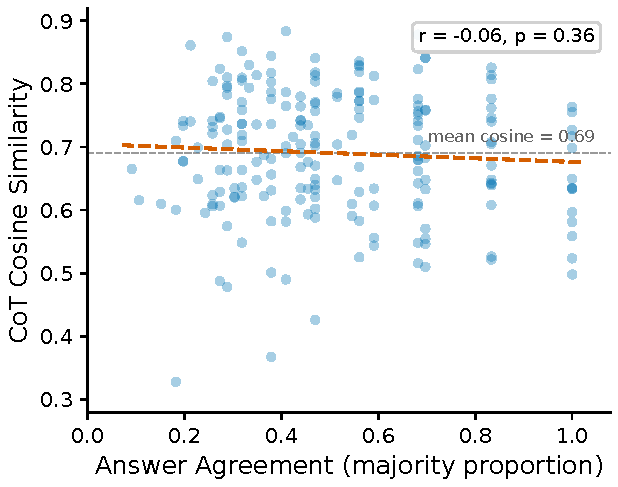
\includegraphics[width=0.85\columnwidth]{figures/fig3_process_kappa_scatter.pdf}
\vspace{-2mm}
\caption{Answer agreement vs.\ CoT cosine similarity (Mistral-7B, FOLIO, $n{=}204$). Flat regression ($r = -0.06$, $p = 0.36$): process and answer independence are uncorrelated.}
\label{fig:process-kappa}
\end{figure}


\subsection{Regime-Dependent Effects}
\label{sec:main-results}
\label{sec:diagnostics}

SICA effectiveness depends sharply on the accuracy regime (Figure~\ref{fig:regime-scatter}).

\paragraph{Intermediate-SC region.} Mistral-7B on FOLIO (SC $\sim$50--60\%) shows positive directional trends in 2 of 4 seeds: $\Delta = +3.43$\,pp ($p = 0.092$) and $+2.94$\,pp ($p = 0.070$); the remaining seeds show null or negative results. No seed reaches $p < 0.05$; the 4-seed mean is $+1.47$\,pp. The default-seed and seed-456 runs share identical SC baselines (55.88\%) yet diverge ($+3.43$ vs.\ $0.00$\,pp), suggesting that seed-level constraint quality, not SC level alone, influences the effect.

\paragraph{Type A (SC $\geq$ 60\%).} All nine Type~A conditions produce no significant positive effects. Even in-context learning with gold logical examples yields $\Delta = +0.50$\,pp (n.s.). Qwen2.5-14B on ProofWriter shows significant degradation ($\Delta = -2.50$\,pp, $p = 0.011$).

\paragraph{Type C (SC $\leq$ 40\%).} Mistral-7B on ProofWriter ($n = 600$, SC $= 39.33\%$) shows $\Delta = -2.83$\,pp ($p = 0.014$): SICA \emph{significantly hurts} by formalizing incorrect reasoning. When $C_0 < 5\%$, nearly all traces agree and SICA reduces to SC by construction.

Four supporting analyses confirm the mechanism: constraint ablation shows both MAX-SAT and count-only each agree with SC on ${>}$96\% of predictions ($n = 804$; Table~\ref{tab:ablation}); 91.8\% of constraints are discriminative but mirror the majority; effects concentrate in high-entropy problems ($+12.8$\,pp) with direction determined by accuracy regime; and hyperparameter peaks coincide with low SC baselines (Appendices~\ref{app:extraction}--\ref{app:entropy}).

\begin{figure}[t]
\centering

\includegraphics[width=\columnwidth]{f2_regime_scatter}
\caption{SICA $\Delta$ (pp) vs.\ SC baseline. Filled: $n \geq 100$; open: $n < 100$. The intermediate-SC region (50--60\%, shaded) contains the only positive trends (none reaching $p < 0.05$). Type~C: significant degradation ($p = 0.014$).}
\label{fig:regime-scatter}
\end{figure}


\subsection{Remediation: 25+ Strategies Fail}
\label{sec:remediation}
\label{sec:interventions}

We test more than twenty remediation strategies spanning prompt engineering, method-level redesign, and ten additional directions. All produce neutral or negative results.

\paragraph{Prompt-level interventions.} Nine strategies spanning six dimensions (Appendix Table~\ref{tab:remediation}) all fail. Contrastive prompting reduces non-discriminative constraints from 8.2\% to 6.0\%, but newly discriminative constraints still mirror the majority ($\Delta = -1.1$\,pp). Cross-model extraction fails in both directions: weaker models yield 0\% discriminative constraints; stronger models produce accuracy within $\pm 1$\,pp of self-extraction. Multi-temperature sampling ($T \in \{0.3, 0.7, 1.2\}$) yields $\Delta = 0.00$\,pp.

\paragraph{Method-level interventions.} ICG ($\Delta \approx 0$, $p = .206$), Contrastive ($\Delta = -9.31$\,pp, $p < 0.01$), and Debate ($\Delta = -18.63$/$-23.00$\,pp, $p < 0.001$) all fail (Table~\ref{tab:method_interventions}, Appendix~\ref{app:remediation}). Ten further experiments (code verification, iterative refinement, logprob filtering, cross-model ensembles) produce neutral-to-negative results (Appendix Table~\ref{tab:additional_interventions}).

\paragraph{Independence-accuracy trade-off.} Table~\ref{tab:kappa_generalization} compares Fleiss' $\kappa$ across four aggregation methods and three model families (Figure~\ref{fig:kappa-accuracy}). SC ($\kappa = 0.44$), Diverse-Prompt ($\kappa = 0.40$), and ICG ($\kappa = 0.47$) cluster at $\kappa \approx 0.40$--$0.47$; Debate reaches $\kappa = 0.15$ but collapses accuracy by $-18.63$\,pp. All three families cluster above $\kappa = 0.40$, forming a same-model trade-off ceiling: methods that increase independence destroy accuracy, and methods preserving accuracy cannot break the correlation floor. Bias ratios exceed $1.0$ across all three families ($4.97\times$ Mistral-7B, $3.85\times$ Qwen2.5-14B, $2.88\times$ LLaMA-3.1-8B); the ordering does not follow a strict capability gradient (LLaMA-3.1-8B shows lower BR than Qwen2.5-14B despite lower SC accuracy). This pattern persists from 7B open-source to frontier closed-source (BR $1.66$--$4.97\times$; Table~\ref{tab:frontier-scb}). For practitioners, $C_0$ combined with SC accuracy predicts when augmentation is unlikely to help: $C_0 < 5\%$ implies degeneration, SC $\geq 60\%$ implies confirmation bias, SC $\leq 40\%$ implies error amplification. Whether trained extractors shift the observed trade-off boundary remains open.

\begin{table}[t]
\centering
\small
\caption{Independence-accuracy trade-off (FOLIO, $n = 204$). Top: aggregation methods on Mistral-7B; bottom: SC across three model families. All families produce $\kappa \geq 0.41$, confirming an architecture-independent ceiling. $\kappa$: Fleiss' kappa on raw answers.}
\label{tab:kappa_generalization}
\setlength{\tabcolsep}{3.5pt}
\begin{tabular}{@{}llccrr@{}}
\toprule
Model & Aggregation & $\kappa$ & Eff-$K$ & $K$ & Acc.\ (\%) \\
\midrule
Mistral-7B & Debate & 0.15 & 4.44 & 12 & 38.24 \\
& Diverse-Prompt & 0.40 & 2.21 & 12 & 54.41 \\
& Self-Consistency & 0.44 & 2.02 & 10 & 56.86 \\
& ICG & 0.47 & 1.93 & 10 & 51.96 \\
\addlinespace
LLaMA-3.1-8B & Self-Consistency & 0.41 & 2.17 & 12 & 66.18 \\
Qwen2.5-7B & Self-Consistency & 0.66 & 1.46 & 12 & 75.98 \\
Qwen2.5-14B & Self-Consistency & 0.74 & 1.32 & 12 & 75.98 \\
\bottomrule
\end{tabular}
\end{table}
